\section{Hardwareentwicklung}
\label{sec:TeilB_Hardware}
In diesem Kapitel wird auf die entwickelte Hardware eingegangen und detailliert dargestellt. Die Abbildungen \ref{fig:teilb_pcb_top} und \ref{fig:teilb_pcb_bot} zeigen die Ober- bzw. Unterseite der 4-Lagigen Platine. In den Bildern sind farblich die einzelnen Bereiche der Platine markiert. 

\begin{table}[h]
\begin{tabular}{|p{8cm}|p{5.5cm}|}\hline
\rowcolor{TableBackgroundColor} 
   \textbf{Bereich auf Platine} & \textbf{Farbe}\\ \hline
  HDMI Eingang &  \textcolor{blue}{Blau} \\ \hline
  RGB Bridge & \textcolor{yellow}{Gelb} \\ \hline
  LVDS Bridge & \textcolor{magenta}{Magenta}  \\ \hline
  EDID-Daten &  \textcolor{orange}{Orange} \\ \hline
  Spannungsversorgung &  \textcolor{green}{Grün} \\ \hline 
\end{tabular}
\caption{Teil B: Farblich gekennzeichnete Bereiche auf der Platine}
\label{tab:pcb_areas}
\end{table}

\begin{figure}[htbp]
        %\begin{center}
        \centering
        \begin{subfigure}[htp]{0.48\textwidth}
                \fbox{\includegraphics[width=1\textwidth]{TeilB/HDMI_RGB_LVDS_V9_top.png}}
                \caption{Top Layer}
                \label{fig:teilb_pcb_top}
        \end{subfigure}
\quad 
        \begin{subfigure}[htp]{0.48\textwidth}
               \fbox{ \includegraphics[width=1\textwidth]{TeilB/HDMI_RGB_LVDS_V9_bot.png} }              				\caption{Bottom Layer}
                \label{fig:teilb_pcb_bot}
        \end{subfigure}
		%\end{center}
        \caption{HDMI RGB/LVDS Board}
        \label{fig:teilb_pcb}
\end{figure}

In den folgenden Abschnitten wird auf die Teilbereiche der Platine im Einzelnen eingegangen. 

\subsection{HDMI-Eingang}
\label{cha:hdmi_eingang}
Der HDMI-Eingang wird durch eine HDMI-Buchse der Firma \code{FCI} realisiert und wird mittels Impedanzkontrollierten Leitungen an die RGB-Bridge weitergegeben. Diese Leitungen sind mit einer differentielle Impedanz von 100 $\Omega$ spezifiziert. Zu beachten ist, dass alle Leitungspaare dieselbe Länge aufweisen, da sonst Laufzeitunterschiede und Fehlabtastung innerhalb der verschiedenen Signalpaare auftreten und zu Fehlern führen können. Die Impedanz der differentieller Leitungen lässt sich nach den Gleichungen 
%
\begin{equation}
Z_0 = \frac{88.75}{\sqrt{\epsilon_r + 1.47}} \cdot ln\left(\frac{5.97 \cdot h}{0.8 \cdot W + t}\right)
\label{equ:z_0}
\end{equation}
%
und
%
\begin{equation}
Z_{Diff} = 2 \cdot Z_0  \cdot \left(1-0.48 \cdot e^{-0.96\frac{s}{h}}\right)
\label{equ:z_diff}
\end{equation}
%
mit den Parametern entsprechend \reft{tab:z_parameter} (siehe \cite{TI2007}). Hier erhält man eine Impedanz $Z_0$ von 77 $\Omega$ und eine differentielle Impedanz von 106 $\Omega$. Aufgrund der kurzen Leitungslängen von maximal 11mm, spielt diese minimale Fehlanpassung keine große Rolle und kann vernachlässigt werden. Die Terminierung findet im Baustein statt und bedarf keiner externen Widerstände an den Enden der Leitungen.
\begin{table}[h]
\begin{tabular}{|p{7cm}|p{3cm}|p{3cm}|}\hline
\rowcolor{TableBackgroundColor} 
   \textbf{Parameter} & \textbf{Bezeichnung} & \textbf{Wert}	\\ \hline
    Dielektrikum 					& $\epsilon_r$	& 4.2		\\ \hline
	Breite der Leitungen  		 	& W 			& 0.28 mm	\\ \hline
	Abstand des Paares zueinander 	& s 			& 0.17 mm 	\\ \hline
	Dicke des Dielektrikums 		& h 			& 0.35 mm 	\\ \hline 
	Dicke der Leiterbahn 			& t 			& 35 µm		\\ \hline 
\end{tabular}
\caption{Teil B: Parameter bezüglich Impedanz der HDMI-Leitungen}
\label{tab:z_parameter}
\end{table} \\
\refa{fig:teilb_hdmi} zeigt den Schaltplan und das Layout des HDMI-Steckeres. In \refa{fig:teilb_hdmi_pcb} sind die TDMS-Leitungspaare zu sehen, bei der der gleichmäßige Abstand zwischen den Leitungen einzelner Paare, sowie die gleiche Länge der Paare selbst eingehalten wird. 


\begin{figure}[htbp]
        %\begin{center}
        \centering
        \begin{subfigure}[htp]{0.48\textwidth}
%			\fbox{	\includegraphics[width=1\textwidth]{TeilB/hdmi_sch.png}}
			\fbox{	\includegraphics[height=6.5cm,width=1\textwidth,keepaspectratio]{TeilB/hdmi_sch.png}}
            \caption{HDMI-Stecker: Schaltplan}
            \label{fig:teilb_hdmi_sch}
        \end{subfigure}
\quad 
        \begin{subfigure}[htp]{0.48\textwidth}
			\fbox{	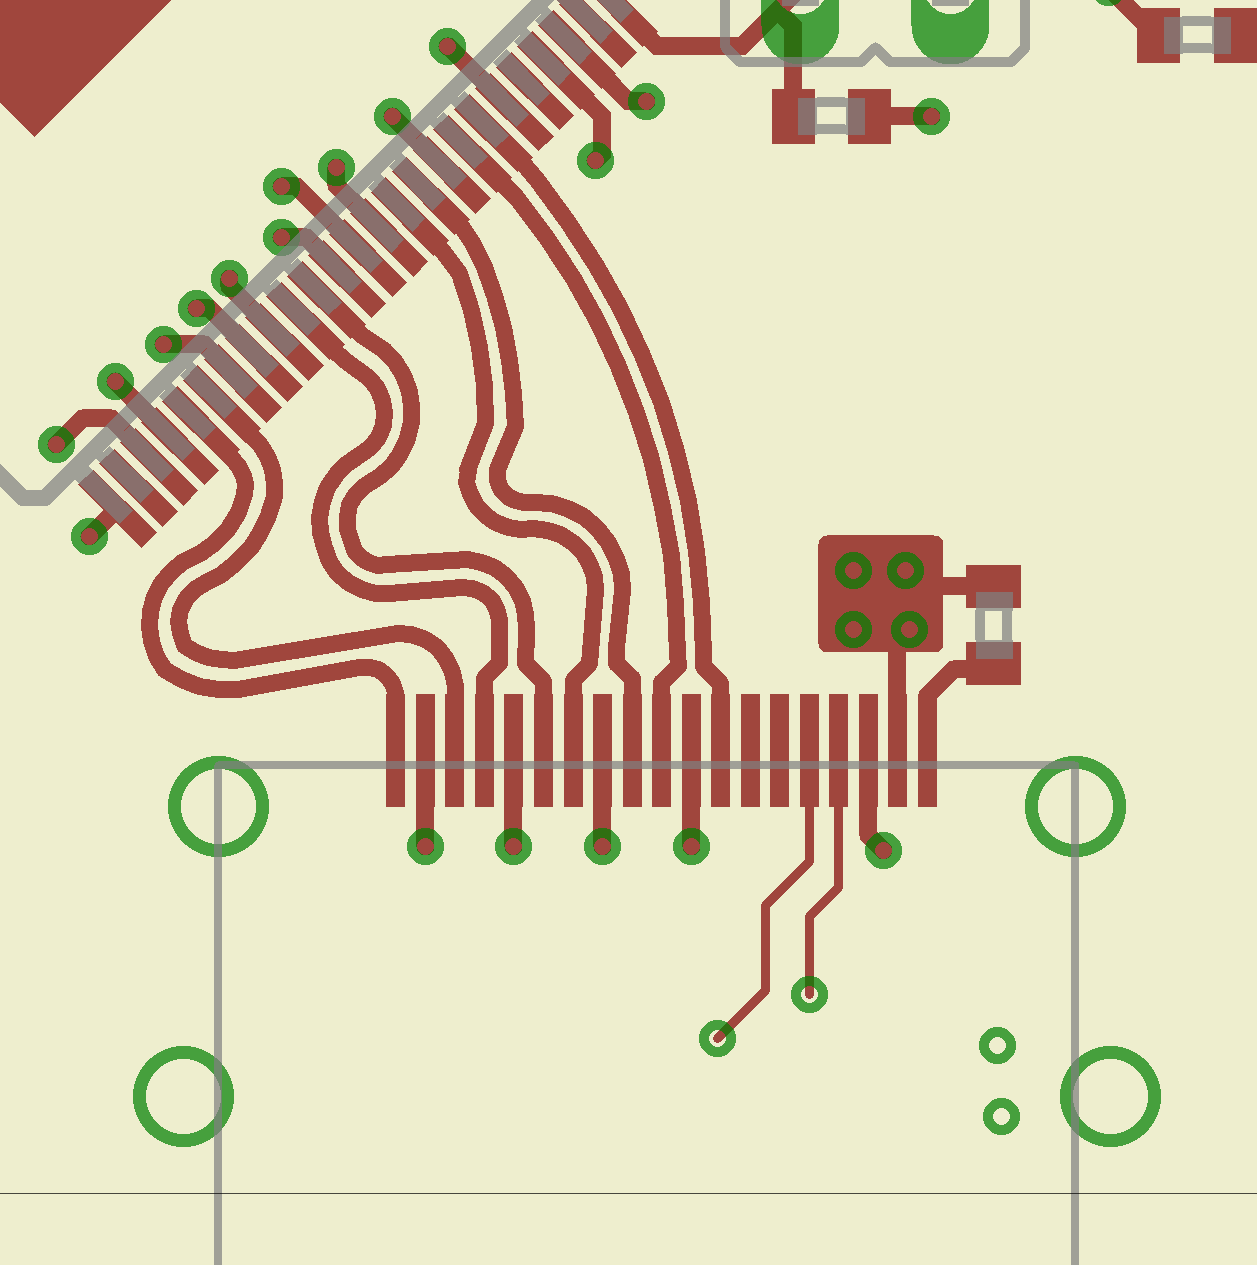
\includegraphics[height=6.5cm,width=1\textwidth,keepaspectratio]{TeilB/hdmi_stecker.png}}
 			\caption{HDMI Stecker: Layout}
            \label{fig:teilb_hdmi_pcb}
        \end{subfigure}
		%\end{center}
        \caption{Teil B: HDMI Leitungen}
        \label{fig:teilb_hdmi}
\end{figure}
Neben den eigentlichen Video-Signalen befinden sich noch die $I^2C$-Signale\footnote{$I^2C$: serieller Zweidraht-Bus} \code{SCL}\footnote{SCL: Taktleitung des $I^2C$-Bus} und \code{SDA}\footnote{SCL: Datenleitung des $I^2C$-Bus} des EDID-EEPROMs sowie eine Hot-Plug-Detection auf der HDMI-Buchse.
\subsection{RGB-Bridge}
Die Eingänge der RGB-Bridge werden vom HDMI-Stecker gespeist. Die TMDS-Signale werden so aufbereitet, dass an den Ausgängen eine RGB-Schnittstelle zum Anschluss eines RGB-Panels bereitgestellt sind.
        \begin{figure}[htp]
        	\center
			\fbox{	\includegraphics[width=0.9\textwidth]{TeilB/rgb_bridge_sch.png}}
%			\fbox{	\includegraphics[width=8.5cm,keepaspectratio]{TeilB/rgb_bridge_sch.png}}
            \caption{RGB Bridge: Schaltplan}
            \label{fig:teilb_rgb_bridge_sch}
        \end{figure}
\newline        
\refa{fig:teilb_rgb_bridge_sch} zeigt den Schaltplan der RGB-Bridge mit dem Stecker für das RGB-Display. Als Baustein ist ein \code{TFP401A} von Texas Instruments im Einsatz. Neben den vier TMDS-Signalpaaren werden eingangsseitig noch die Signale \code{HDMI_PIXS} und \code{HDMI_OCK_INV} eingespeist. Diese sind zur Konfiguration der RGB-Ausgangssignale vorhanden. \\
Ausgangsseitig sind die drei Farbkanäle für Rot, Grün und Blau (\code{RGB_EVEN_R[7:0]}, \code{RGB_EVEN_G[7:0]} und \code{RGB_EVEN_B[7:0]}) sowie die Steuersignale \code{RGB_ODCK}, \code{RGB_DE}, \code{RGB_HSYNC} und \code{RGB_VSYNC} verbunden.
Fließen Ströme mit hoher Frequenz, entstehen aufgrund des Induktionsgesetzes Störeffekte auf den Leitungen, die wiederum andere Signale beeinflussen können. Die induzierte Störspannung lässt sich mit der Gleichung
%
\begin{equation}
u \approx L \cdot \frac{di}{dt}
\label{equ:z_0}
\end{equation}
%
berechnen. Steigt die Schaltfrequenz, und damit die Frequenz der Stromänderung $\frac{di}{dt}$, wird die abgestrahlte Störung ebenfalls stärker. Um diesem Effekt entgegenzuwirken, sind Serienwiderstände im Signalweg eingebaut, die mit der natürlichen Kapazität der Leitung den Tiefpasscharakter der Leitung besser ausprägt. Die Kapazität einer Mikrostreifenleitung lässt sich mit 
%
\begin{equation}
C_{Leiterbahn} = \epsilon_0 \cdot \epsilon_r \cdot \frac{(a+b) \cdot l}{d}
\label{equ:z_0}
\end{equation}
%
mit $\epsilon_0 = 8.86\cdot10^{-12} \frac{Am}{Vs}$, $\epsilon_r = 4.2$, der Leiterbahnbreite $a = 0.15 $mm, der Leiterbahndicke $b = 35$ µm, dem Abstand zur nächsten Fläche $d = 0.35$ mm und der durchschnittlichen Leiterbahnlänge $l = 50$ mm berechnen (siehe \cite{Gensicke2014}). Die durchschnittliche Kapazität der RGB-Leitungen beträgt somit rund 1 pF. In Verbindung mit dem verwendeten 22 $\Omega$ Widerstand bildet dieser in Verbindung mit der Leitung einen Tiefpass. Der quantitative Verlauf des Tiefpass deutet sich in \refa{fig:teilb_tiefpass_mess} an, wobei Grün die originale und Blau die gefilterte Kurve darstellt. Zu erkennen ist, dass die Steilheit der fallenden und steigenden Flanke abnimmt, was zu einer verlangsamten Stromänderung $\frac{di}{dt}$ führt.
\begin{figure}[htbp]
%        %\begin{center}
%        \begin{center}
%        \begin{subfigure}[htp]{1\textwidth}
			\fbox{	\includegraphics[width=1\textwidth,keepaspectratio]{TeilB/sim_serienwiderstand_messung.png}}
 			\caption{RGB Bridge: Messergebnis des Leitungstiefpass}
            \label{fig:teilb_tiefpass_mess}
%        \end{subfigure}
%        \begin{subfigure}[htp]{0.48\textwidth}
%%			\fbox{	\includegraphics[width=1\textwidth]{TeilB/sim_serienwiderstand.png}}
%			\fbox{	\includegraphics[width=1\textwidth,keepaspectratio]{TeilB/sim_serienwiderstand.png}}
%            \caption{RGB Bridge: Simulationsaufbau des Leitungstiefpass}
%            \label{fig:teilb_tiefpass_sim}
%        \end{subfigure}
%%\quad 
%
%		\end{center}
%		%\end{center}
%        \caption{Teil B: Leitungstiefpässe der RGB-Leitungen}
%        \label{fig:teilb_tiefpass}
\end{figure}
\newpage
Das Layout der RGB-Signale, gezeigt in \refa{fig:teilb_rgb_bridge_pcb}, ist unkritischer als das der HDMI-Signale, da beim verwendeten Display ein maximaler Pixeltakt von 33 MHz auftritt (siehe \cite{LG2012}, S.14). Aufgrund der noch relativ langsamen Taktung, haben eventuell auftretende Laufzeitunterschiede zwischen den Signale einen vernachlässigbaren Effekt. Die Serienwiderstände sind als Widerstands-Array mit je vier realisiert.
\begin{figure}[htp]
	\center
	\fbox{\includegraphics[height=0.8\textwidth,keepaspectratio,angle=90]{TeilB/rgb_bridge_pcb.png}}
 	\caption{RGB Bridge: Layout, gedreht um 90$^{\circ}$} 
    \label{fig:teilb_rgb_bridge_pcb}
\end{figure}

\subsection{LVDS-Bridge}
Die LVDS-Bridge teilt die am Eingang liegenden parllelen RGB-Signale in Pakete zu je acht Bit auf und übertragt diese seriell über die verfügbaren LVDS-Kanäle. Die Beschaltung der LVDS-Bridge ist daher auf das verwendete Display \code{LB070WV8-SL01} zugeschnitten und analog den Abbildungen \ref{fig:teilb_lvds_bridge_format} und \ref{fig:teilb_lvds_display_format} zu verbinden.
\begin{figure}[htbp]
        %\begin{center}
        \begin{center}
        \begin{subfigure}[htp]{0.48\textwidth}
			\fbox{	\includegraphics[height=3.3cm]{TeilB/lvds_bridge_paket.png}}
 			\caption{Paketformat LVDS-Bridge, \cite{TI2011b}}
            \label{fig:teilb_lvds_bridge_format}
        \end{subfigure}
        \quad
        \begin{subfigure}[htp]{0.48\textwidth}
			\fbox{	\includegraphics[height=3.3cm]{TeilB/lvds_display_paket.png}}
            \caption{Paketformat LVDS-Display, \cite{LG2012}}
            \label{fig:teilb_lvds_display_format}
        \end{subfigure}
		\end{center}
        \caption{Teil B: LVDS Paketformate}
        \label{fig:teilb_lvds_format}
\end{figure} \\
So liegt zum Beispiel das RGB Bit G4 auf dem Dateneingang D13 der LVDS-Bridge. Der Schaltplan in \refa{fig:teilb_lvds_bridge_sch} zeigt die Beschaltung der LVDS-Bridge und des Steckverbinders für das Display.\\
\begin{figure}[htp]
		\center
		\fbox{	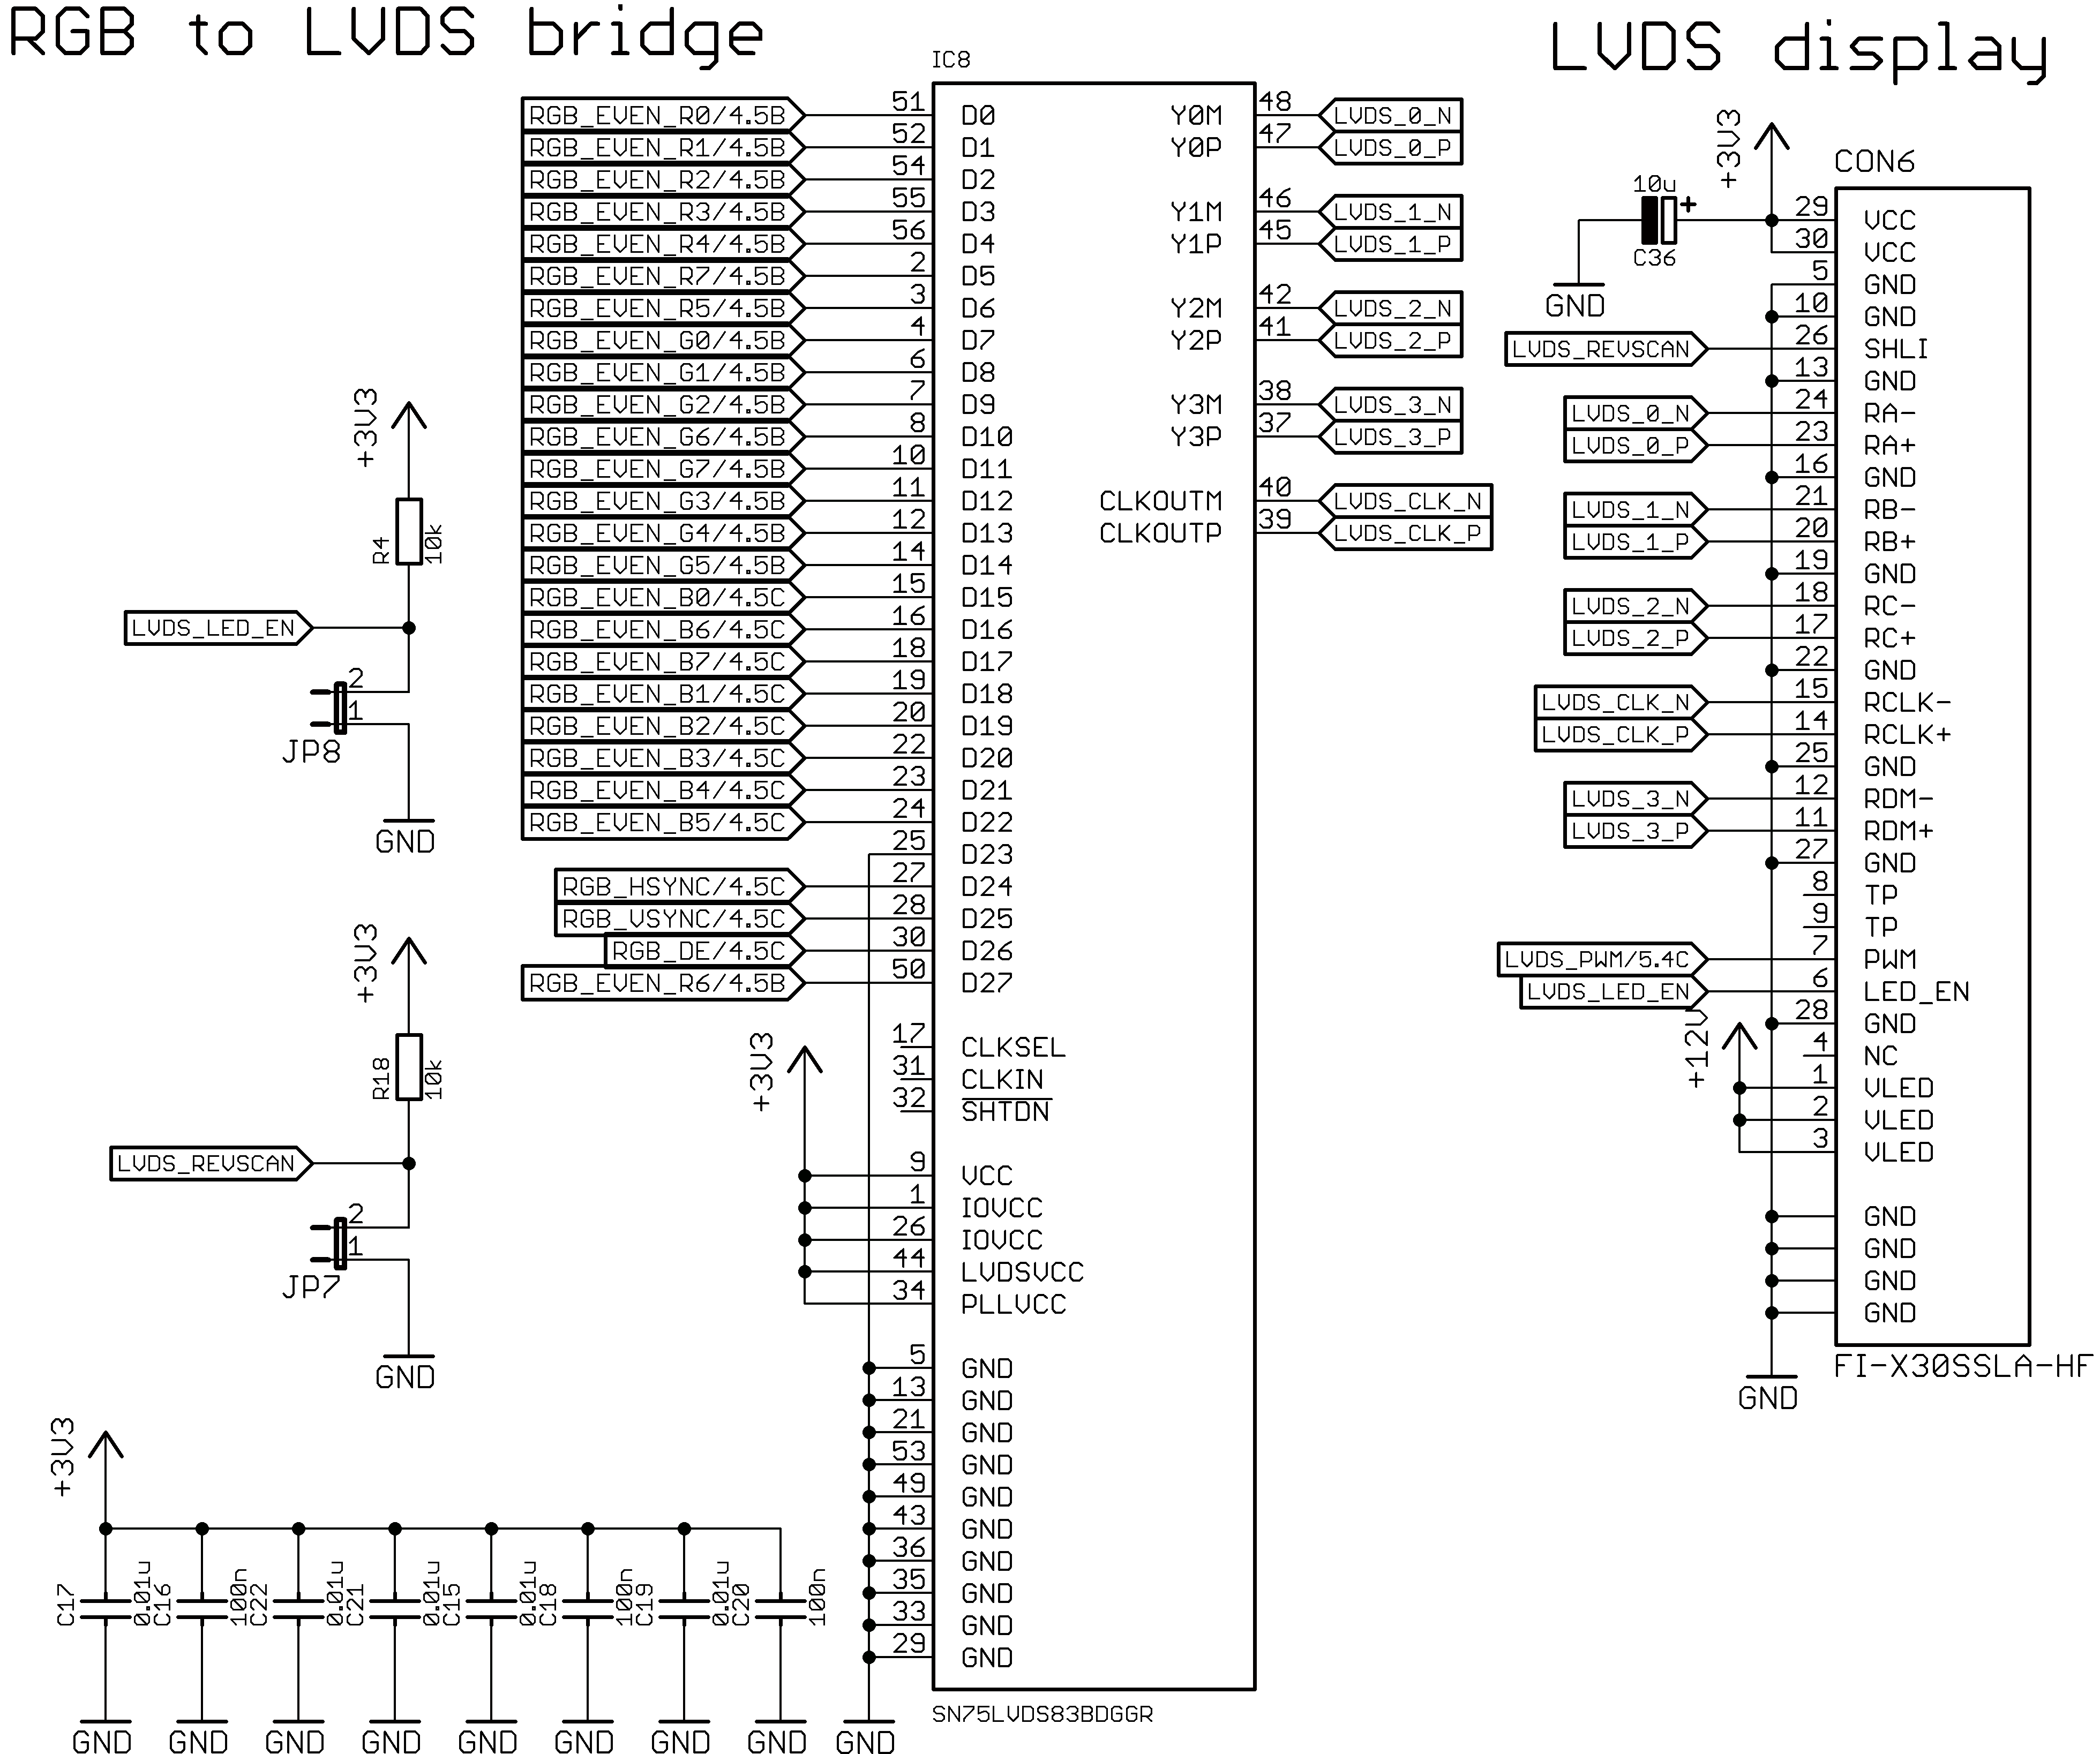
\includegraphics[width=0.8\textwidth]{TeilB/lvds_bridge_sch.png}}
%			\fbox{	\includegraphics[width=8.5cm,keepaspectratio]{TeilB/rgb_bridge_sch.png}}
        \caption{LVDS Bridge: Schaltplan}
       \label{fig:teilb_lvds_bridge_sch}
\end{figure}\\
Wie auch bei den HDMI-Leitungen muss beim Layouten ein besonderes Augenmerk geworfen werden. Da hier ebenfalls eine Impedanz von 100 $\Omega$ gefordert werden, sind dieselben Parameter bzgl. Leitungsbreite und Abstand wie in Abschnitt \ref{cha:hdmi_eingang} verwendet, bei der sich eine differentielle Impedanz von 106 $\Omega$ errechnet.  Die Terminierung findet am Ende der LVDS-Leitungen im Display statt und bedarf keiner zusätzlichen Bauteile auf der Platine. Wie zuvor ist die Länge der Leitungspaare zueinander enorm wichtig. Die Längen der Leitungspaare sind im Bereich zwischen 13.825 mm und 14.010 mm, was einer maximalen Abweichung von 1.34 \% entspricht. Durch die gut angepasste differentielle Impedanz und gleichlangen Leitungen, ist die LVDS-Strecke hinreichend gut dimensioniert. \refa{fig:teilb_lvds_bridge_pcb} zeigt das Layout der LVDS-Bridge. Um die RGB-Signale vom Top-Layer auf den Bottom-Layer zu bekommen, werden diese mit Vias\footnote{Via: Durchkontaktierung um Leitung von einer Lage zu einer anderen zu verbinden} durchkontaktiert. Um große Wege für Rückströme zu verhindern, ist zwischen den Durchkontaktierungen ausreichend Platz, sodass die Vias vollständig von einer Ground-Fläche umschlossen werden.
\begin{figure}[htp]
		\center
		\fbox{	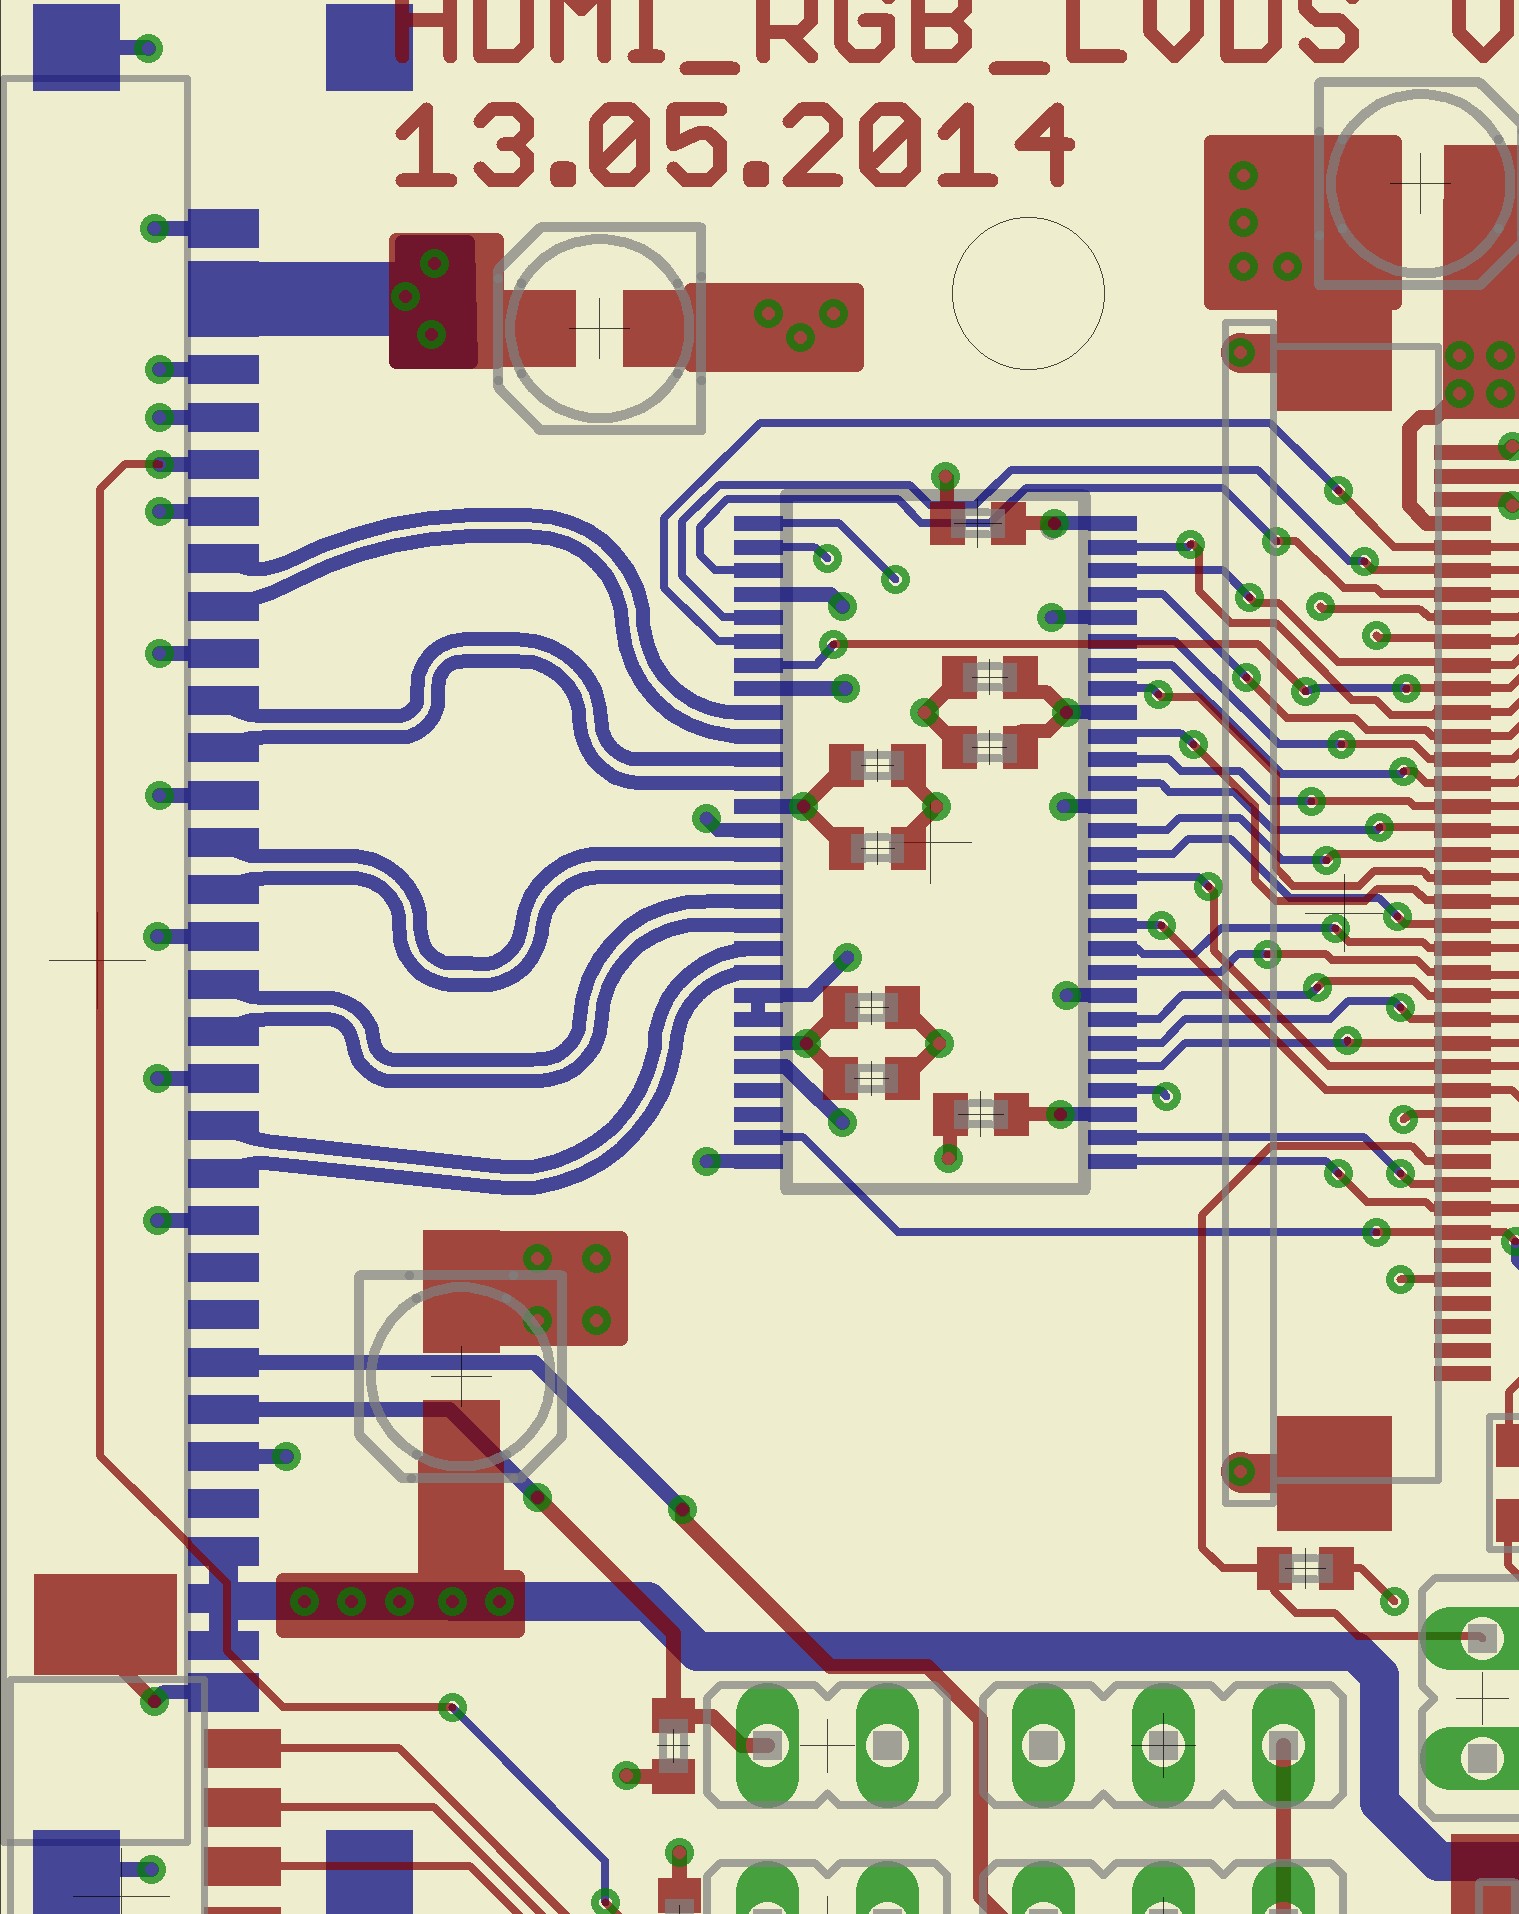
\includegraphics[width=0.8\textwidth]{TeilB/lvds_bridge_pcb.png}}
%			\fbox{	\includegraphics[width=8.5cm,keepaspectratio]{TeilB/rgb_bridge_sch.png}}
        \caption{LVDS Bridge: Layout}
       \label{fig:teilb_lvds_bridge_pcb}
\end{figure}
\newpage


\subsection{EDID-Daten}
\subsection{Spannungsversorgung}
